\documentclass{report}
\usepackage{graphicx}
\usepackage{lmodern}
\usepackage[utf8]{inputenc}
\usepackage{url}
\usepackage{amssymb}
\usepackage{amsmath}
\usepackage{parskip}
\usepackage{listings}
\usepackage{verbatim}
\usepackage{hyperref}
\usepackage{color}

\hypersetup{
    colorlinks,%
    citecolor=black,%
    filecolor=black,%
    linkcolor=black,%
    urlcolor=black
}

% Set up listings to print the code in a snazzy way
\lstdefinelanguage{guardcmd}{morecomment=[l][commentstyle]{//},
		morecomment=[s][commentstyle]{/*}{*/},
		morecomment=[n][commentstyle]{\#},
		morekeywords={skip, abort, if, fi, do, od, module, end, read, write}
}
\lstset{
language=guardcmd,
basicstyle=\footnotesize,       % the size of the fonts that are used for the code
numbers=left,                   % where to put the line-numbers
numberstyle=\footnotesize,      % the size of the fonts that are used for the line-numbers
stepnumber=1,                   % the step between two line-numbers. If it is 1 each line will be numbered
numbersep=5pt,                  % how far the line-numbers are from the code
backgroundcolor=\color{white},  % choose the background color. You must add \usepackage{color}
showspaces=false,               % show spaces adding particular underscores
showstringspaces=false,         % underline spaces within strings
showtabs=false,                 % show tabs within strings adding particular underscores
frame=single,                   % adds a frame around the code
tabsize=2,              % sets default tabsize to 2 spaces
captionpos=b,                   % sets the caption-position to bottom
breaklines=true,        % sets automatic line breaking
breakatwhitespace=false,    % sets if automatic breaks should only happen at whitespace
escapeinside={\%}{)}          % if you want to add a comment within your code
}


\newcommand{\email}[1]{{\href{#1}{#1}}}

\title{Program Analysis 02242 - Guarded Command Language}
\author{Niels Thykier, s072425 (\email{s072425@student.dtu.dk})
\\Melvin Winstrøm-Møller, s072435 (\email{s072435@student.dtu.dk})
\\Morten Sørensen, s072440 (\email{s072440@student.dtu.dk})}

\begin{document}
\parindent 0pt
\parskip 3mm
\setlength{\parindent}{0.5cm}
\newcommand{\docpar}[0]{\vspace{0.5cm} \noindent}
\newcommand{\footref}[1]{\footnotemark[\ref{#1}]}
\newcommand{\newconcept}[1]{\textit{#1}}
\newcommand{\command}[1]{\textbf{#1}}

\maketitle
\phantomsection
\addcontentsline{toc}{section}{Table of Contents}
\tableofcontents
\newpage

\chapter{Introduction}


This report documents a project regarding the
Guarded Command Language (GCL), presented in the course 02242
Program Analysis, DTU, in the fall of 2010.
The project goal is to design, implement and test
a program analysis for GCL, including a parser,
worklist algorithm, several analyses and transformations.
As part of the project, a comparison between the Succint Solver
presented in the course and the implemented worklist algorithm
must be made and documented.
The project has been implemented in Java.




\chapter{Analysis}

\section{General definitions}
When arguing for the correctness of algorithms, defining the flow and labels of the language is
valuable. Below different definitions and functions is given, mirroring those of chapter 2 of the
book given in the course. These include init(C), final(C), blocks(C), labels(C) and flow(C).
Note that C is used instead of S to indicate commands instead of statements, and that
x and y typically denotes variables, and a and e expressions, though this is not always followed.

In the following, the guarded commands are a part of the domain of commands.

\subsection{Termination}

An important point in regards to the flow is whether or not the program is terminated
at a certain point. For instance, the program may terminate at an if, but is not
certain to do so. On the other hand, an abort is certain to terminate, and no flow
occurs in a command that looks like: abort; C$_2$. To get a precise analysis, termination
may be considered. However, since this represents a complication, abort is not guaranteed
to be considered everywhere. In the cases where abort is not considered, the below analysis
can still be applied: replace any occurrence of ``abort'' in the program with ``skip''.
This simplifies the analysis, but makes it less precise.

\subsection{Labelling}

A label is given to every elementary block ``el''. The elementary blocks consists of
the commands assign, skip, abort, read, write, and test. Furthermore, a label is given
to if and do, to simplify definitions later. For all intentions and purposes, the
label of if and do can be seen as being the label of a skip elementary block.

\subsection{Helper functions}

Some helper functions:

guards([e]$_l$ $\to$ C)      = \{[e]$_l$\} \newline
guards(gC$_1$ [] gC$_2$)= guards(gC$_1$) $\cup$ guards(gC$_2$)\newline

\subsection{Init}

init(C) denotes the entry point for the flow of a command.
For instance, the entry point of C$_1$ ; C$_2$ is equal to init(C$_1$),
since C$_1$ contains the entry point. The domain is:
\[init \colon Command \to Label\]
It should be noted that the domain is different from that of the book.

init(C):\newline
init([x := a]$_l$)      = l\newline
init([skip]$_l$)        = l\newline
init([abort]$_l$)       = l\newline
init([read x]$_l$)      = l\newline
init([write a]$_l$)     = l\newline
init(C$_1$; C$_2$)        = init(C$_1$)\newline
init(\{C\})             = init(C)\newline
init([if]$_l$ gC fi)        = l\newline
init([do]$_l$ gC od)        = l\newline

The reasoning behind not simply defining the entry point of an if or a do as the first
test in that if or do is that not only the first test, but all the tests, are entry points.
Thus, simply choosing the first label would be wrong. One way to include all tests would
be to extend the definition of init to map to the powerset of all labels, but this
can complicate the analysis later. Instead, all the tests are included by labelling
the if and do.



\subsection{Final}

final(C) denotes the exit points for the flow of a command.
For instance, the exit point of [read x]$_l$ is l. The domain is:
\[final \colon Command \to \mathcal{P}(Label)\]

\docpar

$final(C):$\\
$final([x := a]_l)     = \{l\}$\\
$final([skip]_l)       = \{l\}$\\
$final([abort]_l)      = \{l\}$\\
$final([read x]_l)     = \{l\}$\\
$final([write a]_l)    = \{l\}$\\
$final(C_1; C_2)		  =
\begin{cases}
(el \vert el \in final(C_1) \wedge el = abort) \cup final(C_2) \textbf{if} (el \vert el \in final(C_1) \wedge el \neq abort) \neq \emptyset \\
(el \vert \in final(C_1) \wedge el = abort) \textbf{else}
\end{cases}$\\
$final(\{C\})          = final(C)$\\
$final(if gC fi)       = final(gC)$\\
$final([do]_l gC od)  = 
guards(gC) \cup (el \vert el \in final(gC) \wedge el = abort)$\\
$final([e]_l \to C)    = final(C)$\\
$final(gC1 [] gC2)      = final(gC1) \cup final(gC2)$\\

\begin{itemize}
\item The reasoning behind the definition of the semicolon command is that the
final commands of C$_2$ will only be reached if there is any flow at all
between C$_1$ and C$_2$: this is not the case if C$_1$ aborts the program
before reaching C$_2$.
\item The reasoning behind the definition of final for if is that the exit points
of an if consists of the final commands in all the commands of the if.
\item The reasoning behind the definition of final for do is that the exit points
of a do consists of all the tests in the do (represented by [do]$_l$)
as well as the final commands that aborts, since the normal final commands
simply flow back to the tests.
\end{itemize}



\subsection{Blocks}

blocks(C) denotes the elementary blocks of a command.
For instance, the elementary blocks of blocks([read x]$_l$) is l. The domain is:
\[final \colon Command \to \mathcal{P}(Elementary Command)\]

\docpar
\begin{equation}
blocks(C):\newline
blocks([x := a]_l)      = {[x := a]_l}\newline
blocks([skip]_l)        = {[skip]_l}\newline
blocks([abort]_l)       = {[abort]_l}\newline
blocks([read x]_l)      = {[read x]_l}\newline
blocks([write a]_l)     = {[write a]_l}\newline
blocks(C_1; C_2)		 = 
\begin{cases}
blocks(C_1) \cup blocks(C_2) \textbf{if} (flow(C_1; C_2) \setminus (flow(C_1) \cup flow(C_2))) \neq \emptyset\\
blocks(C_1) \textbf{else}
\end{cases}
\newline
blocks(\{C\})             = blocks(C)\newline
blocks(if gC fi)        = blocks(gC)\newline
blocks(do gC od)        = blocks(gC)\newline
blocks([e]_l \to C)      = \{[e]_l\} \cup blocks(C)\newline
blocks(gC_1 [] gC_2)= blocks(gC_1) \cup blocks(gC_2)\newline
\end{equation}

The reasoning behind the definition of the semicolon command is that the
blocks function only includes those commands that may be reached. If there is
no flow from C$_1$ to C$_2$, the blocks in C$_2$ will never be reached, and is
therefore never included.



\subsection{Flow}

Flow denotes the possible transitions between elementary blocks.
For instance, the flow of flow(skip[l$_1$]; skip[l$_2$]) is equal to
(l$_1$, l$_2$), since the program would simply transition from the first
skip to the last skip. The domain is:
\[flow \colon Command \to \mathcal{P}(Label)\times\mathcal{P}(Label)\]

flow(C):\newline
flow([x := a]$_l$)        =$\emptyset$\newline
flow([skip]$_l$)          =$\emptyset$\newline
flow([abort]$_l$)         =$\emptyset$\newline
flow([read x]$_l$)        =$\emptyset$\newline
flow([write a]$_l$)       =$\emptyset$\newline
flow\-between(C$_1$, C$_2$)= ((el$_1$, el$_2$) $\vert$ el$_1$ $\in$ final(C$_1$) $\wedge$ el$_1$ $\neq$ abort $\wedge$ el$_2$ $\in$ init(C$_2$))\newline
flow(C$_1$; C$_2$)		 = 
\begin{equation}
\begin{cases}
flow(C_1) \cup flow(C_2) \cup flow-between(C_1, C_2) \textbf{if} flow-between(C_1, C_2) \not = \emptyset\\
flow(C_1) \textbf{else}
\end{cases}
\end{equation}\newline
flow(\{C\}) = C\newline

flow([if]$_l$ gC fi) = ((el$_1$, el$_2$) $\vert$ el$_1$ = [if]$_l$ $\wedge$ el$_2$ $\in$ guards(gC))\newline
$\cup$ flow(gC)\newline

flow([do]$_l$ gC od) = ((el$_1$, el$_2$) $\vert$ el$_1$ = [do]$_l$ $\wedge$ el$_2$ $\in$ guards(gC))\newline
$\cup$ flow(gC)\newline
$\cup$ ((el$_1$, el$_2$) $\vert$ el$_1$ $\in$ final(gC) $\wedge$ el$_1$ $\neq$ abort $\wedge$ el$_2$ $\in$ guards(gC))\newline

flow([e]$_l$ $\to$ C)      = \{([e]$_l$, init(C))\} $\cup$ flow(C) \newline
flow(gC$_1$ [] gC$_2$)= flow(gC$_1$) $\cup$ flow(gC$_2$)\newline


\begin{itemize}
\item The reasoning behind the definition of the semicolon command is that there
is only flow from C$_1$ to C$_2$ if C$_1$ does not abort in all final statements.
\item The reasoning behind the definition of flow for if is that the flow should
flow through the guards, from each guard to its command, and flow through the command.
\item The reasoning behind the definition of flow for do is that the flow should flow
like for if, except that it should flow back to the do label. This is because the do loops,
unlike the if.
\end{itemize}




\section{Reaching Definitions}

In this section, Reaching Definitions (RD) analysis will be defined.
RD is a forward-may analysis, that indicates where variables may have
been assigned at any given point. Given that it is a may analysis,
it may include assignments which actually does not reach the given point.
For an imprecise analysis, this is easy to see in the example program;
x := a; abort; skip. An analysis is allowed to let the assignment to x
reach the skip, which is imprecise. To increase the precision of the analysis,
this definition of RD kills the assignment to x before it reaches the skip.

In regards to RD, the definitions is the same as the book given for the course,
except for the kill and gen functions. These will be defined below.
After the definitions, example programs and analysis will be given.

\subsection{Kill}

The definition of kill is the mapping from elementary blocks to the set of variable-label pairs
that are removed by the elementary block. The domain is:
\[final \colon Elementary Command \to \mathcal{P}(Variable)\times\mathcal{P}(Label)\]

kill$_{RD}$(C):\newline
kill$_{RD}$([x := a]$_l$)           = \{(x, ?)\} $\cup$ ((x, l') $\vert$ B$_l$' is an assignment to x in C*)\newline
kill$_{RD}$([read x]$_l$)           = \{(x, ?)\} $\cup$ ((x, l') $\vert$ B$_l$' is an assignment to x in C*)\newline
kill$_{RD}$([skip]$_l$)             =$\emptyset$\newline
kill$_{RD}$([abort]$_l$) 			= ((x, l) $\vert$ l $\in$ labels(C*) and x $\in$ FV(C*) )\newline
kill$_{RD}$([write a]$_l$)          =$\emptyset$\newline
kill$_{RD}$([if]$_l$ gC fi)         =$\emptyset$\newline
kill$_{RD}$([do]$_l$ gC od)         =$\emptyset$\newline
kill$_{RD}$([e]$_l$)                =$\emptyset$\newline

Note that the abort kills everything.

\subsection{Gen}

The definition of gen is the mapping from elementary blocks to the set of variable-label pairs
that are added by the elementary block. The domain is:
\[final \colon Elementary Command \to \mathcal{P}(Variable)\times\mathcal{P}(Label)\]

gen$_{RD}$(C):\newline
gen$_{RD}$([x := a]$_l$)           = \{(x, l)\}\newline
gen$_{RD}$([read x]$_l$)           = \{(x, l)\}\newline
gen$_{RD}$([skip]$_l$)             =$\emptyset$\newline
gen$_{RD}$([abort]$_l$) 			= $\emptyset$\newline
gen$_{RD}$([write a]$_l$)          =$\emptyset$\newline
gen$_{RD}$([if]$_l$ gC fi)         =$\emptyset$\newline
gen$_{RD}$([do]$_l$ gC od)         =$\emptyset$\newline
gen$_{RD}$([e]$_l$)                =$\emptyset$\newline

\subsection{Examples}

Example 1:

\begin{lstlisting}
module rd-example :
read x;[1]
if (x > 0)[2]
  -> y := 0[3]; skip[4]
[] x <= 0[5]
  -> y := 1[6]; abort[7]
fi;
i := 0;[8]
do (i < 10)[9]
  i := i + 1[10]
od
end
\end{lstlisting}
gives as entry for label 8:
\[RD_{entry}(8) = \{(x, 1), (y, 3), (i, ?)\}\]
and exit:
\[RD_{exit}(8) = \{(x, 1), (y, 3), (i, 8)\}\]

For label 10, entry:
\[RD_{entry}(10) = \{(x, 1), (y, 3), (i, 8), (i, 10)\}\]
and exit:
\[RD_{exit}(10) = \{(x, 1), (y, 3), (i, 10)\}\]






\section{Live variable}

//TODO: Niels

In this section, Live Variable (LV) analysis (LVA) will be defined.
LVA is a backwards-may analysis, that indicates which variables are
alive at each command: A variable is alive if there is some path
from the label to a use of the variable that does not redefine it.

  A simple example is: x := a; x := b; x := c; write x.
Here, x is dead at the two first commands, since it is redefined
before it is read. Note that variables that are never read will
automatically be dead. By detecting superfluous defines, LV
can be used to remove dead code.

In regards to LV, the definitions is the same as the book given for the course,
except for the kill and gen functions. These will be defined below.
After the definitions, example programs and analysis will be given.

\subsection{Kill}

The definition of kill is the mapping from elementary blocks to the set of variables
that are removed by the elementary block. The domain is:
\[final \colon Elementary Command \to \mathcal{P}(Variable)\]

\docpar
kill$_{LV}$(C):\newline
kill$_{LV}$([x := a]$_l$)           = \{x\}
kill$_{LV}$([read x]$_l$)           = \{x\}
kill$_{LV}$([skip]$_l$)             = $\emptyset$\newline
kill$_{LV}$([abort]$_l$) 			= FV(C*)\newline
kill$_{LV}$([write a]$_l$)          =$\emptyset$\newline
kill$_{LV}$([if]$_l$ gC fi)         =$\emptyset$\newline
kill$_{LV}$([do]$_l$ gC od)         =$\emptyset$\newline
kill$_{LV}$([e]$_l$)                =$\emptyset$\newline

Note that the abort kills everything, since x will clearly not survive to the write in
x := a; abort; write x, and is therefore dead at the write.

\subsection{Gen}

The definition of gen is the mapping from elementary blocks to the set of variables
that are added by the elementary block. The domain is:
\[final \colon Elementary Command \to \mathcal{P}(Variable)\]

\docpar
gen$_{LV}$(C):\newline
gen$_{LV}$([x := a]$_l$)           = FV(a)\newline
gen$_{LV}$([read x]$_l$)           = $\emptyset$\newline
gen$_{LV}$([skip]$_l$)             = $\emptyset$\newline
gen$_{LV}$([abort]$_l$) 		   = $\emptyset$\newline
gen$_{LV}$([write a]$_l$)          = FV(a)\newline
gen$_{LV}$([if]$_l$ gC fi)         = $\emptyset$\newline
gen$_{LV}$([do]$_l$ gC od)         = $\emptyset$\newline
gen$_{LV}$([e]$_l$)                = FV(e)\newline

\subsection{LV, Faint variables and Strongly Live Variables}
LVA is like RDA a member of the bit-vector analyses. This has some advantages
in terms of simplicity, such as all operations can be specified as trivial
kill and gen functions.
  Unfortunately it turns out this simplicity of LVA has a price, namely that
it sometimes considers variables live that are in fact dead. These variables
are referred to as ``Faint Variables''.
  Faint variables appear because gen does not consider the relevance of the
variable being assigned to; thus it will always consider all variables in
the expression to be alive. Non-faint live variables are sometimes also referred
to as ``Strongly Live Variables''.

\docpar
Trivial analysis of LVA shows that it is possible to upgrade the algorithm into
ignoring faint variables; this upgraded algorithm is sometimes called ``Strongly
Live Variables Analysis'' (SLVA). The upgrade is conditionally using gen on
assignment statements; that is:

\docpar
gen$_{LV}$([x := a]$_l$)           = FV(a)\newline

\docpar
becomes:

\docpar
gen$_{LV}$([x := a]$_l$)           = $$\begin{cases}
$FV(a) if x is live$\\
\emptyset$ else$
\end{cases}
$$\newline

\docpar
The unfortunate side effect of this is that SLVA is not a true bit-vector
analysis. Nevertheless, even with the change it is still a part of the
monotone framework, so using SLVA is not an issue.

\subsection{Examples}
These examples will demonstrate how LVA and SVLA work; for the sake of
clarification strongly live variables will be written in bold
(e.g. \textbf{y}) to separate them from the faint variables.

\docpar
Example 1:
\begin{lstlisting}
module lv-example-1 :
x := 10;[1]
x := 5000;[2]
x := a;[3]
write y[4]
\end{lstlisting}
The entry value of [4] is the empty set; its
exit value is 
\[ SLV_{exit}(4) = LV_{exit}(4) = \{\textbf{y}\}\]
The entry value of [3] is trivially equal to the
exit value of [4]. But in [3] LVA is unable to see
that since x is dead, then a should not be
generated. So a is added as a faint variable:

\[LV_{exit}(3) = \{a, \textbf{y}\}\]

On the other hand SLVA will be able to tell and thus
when using SLVA, the exit value will be:

\[SLV_{exit}(3) = \{\textbf{y}\}\]

Continuing with the analysis it turns out that the
entry and the exit value of [1] and [2] is just the
exit value of [3]. Looking at the results then the
data from LVA makes it possible to remove [3].
In comparison the data from SLVA will also mark [1]
and [2] as redundant.
  After removing [3], it is possible to rerun LVA
and conclude now that [1] and [2] are also redundant.

\docpar
Example 2:
\begin{lstlisting}
module lv-example-2 :
x := z;[1]
if (z > 0)[2] -> x := -1[3]
[] (z <= 0)[4] -> x := 1[5]
fi;
write x*127[6]
\end{lstlisting}




\section{Constant propagation}
There are different views on what exactly constant propagation (CP) means. In its
strictest meaning it is read as ``propagate constants and nothing else''.
However it could also be ``fold constants and then propagate'', which is what
some people use.

  The difference is important and can be demonstrated with the following little
piece of code:

\begin{lstlisting}
module cp-definition :
a := 1;[1]
b := a + 1;[2]
c := a;[3]
write b[4]
\end{lstlisting}

If we only propagate constants then the analysis will conclude that all instances
of a can be replaced by 1 and from [3] on, this will also hold for c. However it
would not be able to give a value for b, since it is not defined to be a 
single constant value.

  If we use the fold-and-propagate method, then it will see that a can be replaced
by 1 in [2] and that it can now fold 1 + 1 to 2 and thus replace b with 2 in [4].
We shall use the fold-and-propagate definition of constant propagation here.

\subsection{Theory}
CP is unlike LV and RD not a part of the bit-vector framework; in fact it is not
even a distributive framework. Thus it cannot be defined by at a kill and a gen
function. Instead we define a complete lattice:

\[ \hat{State}_{cp} = ((V, (Var_{*} \rightarrow \mathbb{Z}^{\top})_\bot), \sqsubseteq, \sqcup, \sqcap, \bot, \lambda x.\top) \]

\docpar
The main difference between our definition and the one Nielson use is the first
element. Namely we use $(V, (Var_{*} \rightarrow \mathbb{Z}^{\top})_\bot)$
compared to Nielson's $(Var_{*} \rightarrow \mathbb{Z}^{\top})_\bot)$; the
reason for this change will become apparent later.
  For those who have not read Nielson's definition, $Var_{*}$ is a set consisting
of all the variables in the program and $\mathbb{Z}^\top$ is the same as
$\mathbb{Z} \cup \{\top\}$. T (also known as ``Top'') is a special value denoting
that the value of the variable is defined, but its exact value cannot be
determined. There is also cases where the variable is simply not defined or
no information is available; in which case we use $\bot$ (also known as
``Bottom''). The result is referred to as:
 $(Var_{*} \rightarrow \mathbb{Z}^{\top})_\bot)$

  We also introduced a $V$ which is defined as $V = true \vee V = false$; which
we will come back to later.  First we will define the partial ordering
$\sqsubseteq$ for our lattice and for that we define $\hat{\sigma}(x)$ to be
whether x is either Top, Bottom or a constant and if it is a constant then
$\hat{\sigma}(x)$ will be that constant. As an exception if $V = false$ then
$\hat{\sigma}(x)$ is always $\bot$.

\docpar
The partial ordering:

\[ \forall{}\hat{\sigma} \in (false, (Var_{*} \rightarrow
 \mathbb{Z}^{\top})_{\bot}): \bot = \hat{\sigma} \]
\[ \forall{}\hat{\sigma} \in (true, (Var_{*} \rightarrow
\mathbb{Z}^{\top})_{\bot}): \bot \sqsubseteq \hat{\sigma} \]
\[ \forall{}\hat{\sigma}_1,\hat{\sigma}_2 \in (true, (Var_{*} \rightarrow
\mathbb{Z}^{\top})_\bot): \hat{\sigma}_2 \sqsubseteq \hat{\sigma}_2 \:
\textbf{iff}  \; \forall{}x : \hat{\sigma}_1(x) \sqsubseteq \hat{\sigma}_2(x) \]

\docpar
The least upper bound is defined as:

\[ \forall{}\hat{\sigma} \in (V, (Var_{*} \rightarrow \mathbb{Z}^{\top})_{\bot}):
 \bot \sqsubseteq \hat{\sigma} = \hat{\sigma} \sqsubseteq \bot = \hat{\sigma} \]
\[ \forall{}\hat{\sigma}_1,\hat{\sigma}_2 \in (V, (Var_{*} \rightarrow
 \mathbb{Z}^{\top})_\bot): \forall{}x : (\hat{\sigma}_1 \sqcup \hat{\sigma}_2)(x) =
 \hat{\sigma}_1(x) \sqcup \hat{\sigma}_2(x) \]

\begin{table}
\[ A_{CP} : \textbf{AExp} \rightarrow (\hat{State}_{CP} \rightarrow \mathbb{Z}^{\top}_\bot) \]
\hrule
\begin{eqnarray}
A_{CP}[x]\hat{\sigma} &=& \begin{cases}
\bot \; if \: \hat{\sigma} = \bot \\
\hat{\sigma}(x) \; otherwise
\end{cases} \\
A_{CP}[n]\hat{\sigma} &=& \begin{cases}
\bot \; if \: \hat{\sigma} = \bot \\
n \; otherwise
\end{cases}\\
A_{CP}[a_1 \; op_a \; a_2]\hat{\sigma} &=& A_{CP}[a_1]\hat{\sigma} \; \hat{op}_a \; A_{CP}[a_2]\hat{\sigma}
\end{eqnarray}
\[ transfer \; functions: f^{CP}_{l} \]
\hrule
\begin{eqnarray}
[x := a]^l : \; \; f^{CP}_l(\hat{\sigma}) &=& \begin{cases}
\bot \; if \hat{\sigma} = \bot \\
\hat{\sigma}[a \mapsto A_{CP}[a]\hat{\sigma}] \; otherwise
\end{cases}\\
\left[skip\right] : \; \; f^{CP}_l(\hat{\sigma}) &=& \hat{\sigma} \\
\left[b\right]^{l} : \; \; f^{CP}_l(\hat{\sigma}) &=& \hat{\sigma}\\
\left[write \; e\right]^{l} : \; \; f^{CP}_l(\hat{\sigma}) &=& \hat{\sigma}\\
\left[read \; x\right]^{l} : \; \; f^{CP}_l(\hat{\sigma}) &=& \hat{\sigma}[a \mapsto \top] \;
\end{eqnarray}
\hrule
\caption{Constant Propagation Analysis}
\end{table}

\docpar
It turns out that our definition of CP for the guarded-command language
have a lot in common as Nielson's definition of CP for the while language
(e.g. the transfer functions are identical for the statements that while
and the guarded-command language share).

  One important difference we have not handled is the abort statement.
The abort statement will set $V$ to false, rendering all the information
in the mapping invalid.

  The idea is that when a statement has an entry value based on the exit
value of two (or more statements), all the ones with $V = false$ will be
ignored, unless all exit values have $V = false$. This is because $V = false$
denotes that the mapping has passed through an abort and therefore does
not represent a valid flow in the program.

\docpar
The $\hat{op}_a$ describes how we operate on values, which are lifted to
 $\mathbb{Z}^{\top}_{\bot} = \mathbb{Z} \cup \{ \top, \bot \}$. The idea is
that if all the values in the operation are defined constants, it can be
computed according to the rules of the operator. That is:

\[ z_1 \hat{op}_a z_2 = z_1 op_a z_2 \; if z_1, z_2 \in \mathbb{Z} \]

\docpar
Otherwise the result is generally either $\bot$ if either $z_1$ or $z_2$
are $\bot$ or else the result is $\top$. There are some special case
exceptions to this rule, such as $0 * z$ or $z - z$, where the result is
0 even if $z$ is $\top$. Though one could argue it is not the job of CP to
conclude the latter.

\subsection{Extension - Branch elimination}
It is possible to extend the constant propagation analysis (CPA) to yield better
results. Consider this example:

\begin{lstlisting}
module cp-ext-el-1 :
x := 0;[1]
if (x > 0)[2] -> y := 1[3]
[] (x = 0)[4] -> y := 0[5]
fi;
write y[6]
\end{lstlisting}

\docpar
It is trivial to see that since x is 0, then only one branch can be taken; namely
the one through [4] and [5]. Thus at [6] y can only be 0. The CP analysis is able
to already conclude when looking at [2] that [3] will only ruin the precision
of the analysis.

  There are some less trivial examples such as this one:

\begin{lstlisting}
module cp-ext-el-2 :
x := 0;[1]
y := 0;[2]
do (x > 0)[3] -> y := y + 1;[4] x := x - 1[5]
[] (x = 0)[6] -> x := -1[7]
do;
write y[8]
\end{lstlisting}

\docpar
Here it is also possible to conclude that y must be 0 at [8], but it is more
difficult. Looking at [3] we know that this branch will not be
taken the first time, but [6] will. This leads us to [7] which sets x to -1
and thus neither [3] nor [6] can evaluate to true any more and the loop will
terminate. Since y has not changed, it retains its value from [2], namely 0.

  This is something that a human will be able to see, but writing a proof for
this that holds for all of these kind of cases is difficult at best.

\docpar
As mentioned this extension will provide better results if implemented correctly
but either the analysis becomes more complicated, since this kind of information
has to be propagated around in the program graph and handled specially when
merging.

  The alternative is to let this extension be an on-the-fly transformation that
removes the flow between two nodes if the analysis concludes it will never pass
through that edge in the graph.



\chapter{Design and implementation}


\section{Data Structure}

The program is translated into a tree-like structure where each node
is either a compound node (having children) or is a leaf node representing
an ``3-address expression''.

  A variation ``3-address expression'' is also used in the ``GIMPLE'' trees,
which is the internal/intermediate representation (IR) used in the GNU Compiler
Collection (GCC) ``middle-end''.

\paragraph*{Leaf nodes}
are all ``simple'' expressions, which are rewritten to 1 or 2 operands expressions. Here
simple refers to any non-compound expression (that is all language constructs
except things like do-od, if-fi and \{\})

In this particular IR all expressions are reduced to 1 or 2 operands expressions.
As an example:

\begin{lstlisting}
	c := a * (b + c) / 4
\end{lstlisting}
	
will be translated to the following leaf nodes:

\begin{lstlisting}
	t1 := b + c
	t2 := a * t1
	c := t2/4
\end{lstlisting}
	
In some cases the IR/the language only allows a single node and in these cases
the nodes are wrapped in a single compound (``SCOPE'') node. In some cases the
IR puts SCOPE nodes in places the language would not allow it, as an example:

\begin{lstlisting}
	if ((x > 3) | (y > 3)) -> skip if
\end{lstlisting}

In this case the guard would be represented as:

\begin{lstlisting}
	{
		t1 := x > 3
		t2 := y > 3
		t3 := t1 | t2
	}
\end{lstlisting}

This is not a problem in this language, because when during the reverse transformation
this scope can trivially be replaced with a bracket group and it will now be a valid
program again.

Finally there also some language constructs that may disappear in the IR. Particularly
brackets will vanish. As seen in the example above, the brackets are not represented at
all. They are used when constructing the IR to order leaf node, but 

//TODO: Ending mid-sentence.

\paragraph*{Compound nodes}
refers to language constructs that contains other nodes. In the IR there are 3 kind of
compund nodes, which are IF, DO and SCOPE. A SCOPE node simply contain a list of nodes
in the order of the flow for that scope. The IF and DO nodes are a little more special.

  The IF and DO node have twice as many child nodes as the original if statement in the
language had branches. One of these nodes represents the guard and the other the command.
The nodes are ordered so that guards comes first and the commands follow. The commands
are inserted in the same order as their guard, so the i'th command is protected by the
i'th guard.

\docpar
A special case is the $module x : y end$ construct. This is represented as a ``compilation
unit'' with a root node. The root node is a SCOPE node containing all the nodes that y
represents. This means that (e.g.) x is not a part of the tree structure.

\subsection{Advantages}
One of the advantages of this format is that everything calculation is reduced to
small simple chunks. It is also possible to trivially transform this into a format
that can be executed by ``3-address instruction'' machine.

A second and very important advantage (and disadvantage) is that the flow becomes
a part of the structure. In a SCOPE the control flows from a node to its sibling
and there is no ``magic'' flow in or out of a SCOPE except for the entry at the
first child and the exit at the last child (modulo ABORT statement; see
Disadvantages about that).

  The implicit flow makes it very easy to see whether or not a statement is inside a
``strongly connected component''. This is important because it is if an analysis reaches
a fixed-point inside one of these components, this component is ``done'' (unless there is
a change in a previous component that flows into this component).

  There are two cases in this representation; if the node is a DO, then the node and
everything below is consists of one strongly connected component. Otherwise each leaf
node is its own strongly connected component. Note that IF and SCOPE changes do not
effect the strength of how connected their children are.

\subsection{Disadvantages}
The representation is not trivial to ``untransform'' into the source language even if no
modifications have been made, particularly due to the great amount of temporary variables
introduced. This also has a consequence for some analyses, since their time
or/and space complexity are (partly) bounded by the number of variables.

  A slightly better variation of this IR might have been to use a tree structure to
describe the operands. This representation would likely have its own issues, but would
allow an easier transformation back to source form (since the original expression is now
fully available in the statement) and it would most likely eliminate the need for the
temporary variables. It was planned to change to this IR, but due to time constrains
it was never started.

\docpar
Since the flow is embedded in the structure, non-standard flow is difficult to handle.
As an example if the language had  ``GOTO'' statements, it would have proved complicated.
One could also argue that ABORT does not have a flow; though in this representation the
analysis will end up ``flowing'' through ABORTs.

  A consequence of this is that analyses have to be able to handle ABORT statements and
define an ``exit value'' of an ABORT statement. On the plus side, it turned out that this
exit value for Constant Propagation Analysis could be (ab)used positively.




\section{Program Slicing}

Please describe program slicing here.



\section{Dead code elimination}
//TODO: Morten



\section{Constant folding}
//TODO: Niels



\chapter{Test}

\section{Program slicing}

Testing of program slicing has been based on two main methods;
Testing by hand, by running the test and considering if the output
is reasonable, and automated testing. Both in the manual and automated
test source code files in the GCL from the different groups have been
used. This has caused some issues, since program slicing is defined
differently for different groups. Therefore, the expectations of the
programs has changed depending on the definition.
Of note is that program slicing in this project is based on a statement
and not specific variables in a statement.

The program slicing examples and test instructions are given in the 
appendix: \ref{ps_test_examples}

\subsection{Test results}

Different tests has been used, including from other groups in the course
of the project. For those files which the files have been modified or the
expected result is different, it is noted.

When the Notes say ``more precise'', it means that this project's program
slicing is more precise, and likewise for ``less precise''.

\begin{tabular}{ |l||l|p{7cm}| }
\hline
  Name & Result & Notes \\
\hline
  example\_1		& Correct &  \\
\hline
  example\_2		& Correct &  \\
\hline
  def\_prog\_1		& Correct & Taken from the design and implementation \\
\hline
  def\_prog\_2		& Correct & .., control flow \\
\hline
  def\_prog\_3		& Correct & .., do, version where S2 affects P.\\
\hline
  def\_prog\_4		& Correct & .., do, version where S2 does not affect P. \\
\hline
  def\_prog\_5		& Correct & .., if. \\
\hline
  def\_prog\_6		& Correct & .., non-termination. \\
\hline
  group2\_1		& Correct &  Very different definition of program slicing.
Group 2 eliminates control flow fully.\\
\hline
  group3\_1		& Correct &  Different definition of program slicing.
Group 3 removes program structure and flow (if, do). But they include the same
conditions and statements which is present in the result of this projects program slicing,
so they must consider the flow as well, indicating the definition is similar.\\
\hline
  group7\_1		& Correct &  Same comments as for group 3.\\
\hline
  group8\_3		& Correct &  Different expectation; more precise\\
\hline
  group9\_1		& Correct &  This project's group.\\
\hline
  group11\_2		& Correct &  Different expectation; less precise,
but it is a special case regarding if, and the statement itself is not included\\
\hline
  group12\_2		& Correct &  Much more precise; group 12's example includes statements
not affeting the loop or the values computed at the given statement.\\
\hline
  group14\_1		& Correct &  Very different definition of program slicing.
Group 14 eliminates control flow fully.\\
\hline
\end{tabular}

\subsection{Conclusion}

Many different tests, including special cases and general programs,
have been sliced, and the implementation have given the correct output
for each. Based on these results, it is concluded that on several
programs, the program slicing implementation produces the correct output.

It is also noted that several groups have different definitions of program slicing.
It is noted that this project seem to have a more useful definition than some
other definitions.
Group 8 has a very similar definition (the groups have also communicated in regards
to a review), and group 3 and 7 seemed to have definitions a little similar.
Other groups had very different definitions, and investigating the usefulness of
those definitions compared to this projects definition may be fruitful in regards
to choosing a definition.



\section{Dead code elimination}

Results of Dead Code Elimination.
All tests have passed, and manual testing have found no errors.
Results and discussion:
\ref{dce_test_results}



\section{Constant folding}

Results of Constant Folding.
All tests have passed, and manual testing have found no errors.
Results:
\ref{cf_test_results}



\section{Succinct Solver}
The succinct solver is a blackbox approach to solve the exact same problems as we have solved with our own implementation. The succinct solver uses Alternation-Free Least Fixed Point Logic (ALFP) to describe the problem and how it should be solved. ALFP is described as follows:

Values:
$v ::= c | x | f(v_1,...,v_k)$

Preconditions:
$pre ::= R(v_1,...v_k) | \neg R(v_1,...,v_k)
      |  v_1 = v_2 | v1 \not= v_2
      |  pre_1 \wedge pre_2 | pre_1 \vee pre_2
      |  \forall x : pre | \exists x : pre$

Clauses:
$cl ::= R(v_1,...,v_k) | true | cl_1 \wedge cl_2
     |  pre \Rightarrow cl | \forall x : cl$

For our test of the succinct solver, we are only going to use RDA for comparison. Additional analysis could be formed using the above clauses if time had permitted it.

\subsection{Succinct solver correctness}
To see the actual clauses in action, the following example can be used. But before the walkthrough of an example, there is a small disclaimer. The clauses generated may not be perfect (as in, formed such that it would help the succinct solver), but immitates the internal representation of everything. This means that temporary variables might occure in the resulting set og clauses which they are not visible in the code from which it is generated from. Also, the labeling does not start from 1 and counts up, but uses the hashcodes of statements that is also used internally.

This is a simple program:
\begin{lstlisting}
module example:
read x;[4d47c5fc]
read y;[4e3eca90]
x := 1;[19c1ea29]
y := (x+2);[4413ee]
write (y);[3597a37c]
\end{lstlisting}
The generated set of clauses will then be:

var(x) \& var(y) \&\newline
label(0) \& label(19c1ea29) \& label(3597a37c) \& label(4413ee) \& label(4d47c5fc) \& label(4e3eca90) \&\newline
flow(4e3eca90,19c1ea29) \& flow(4d47c5fc,4e3eca90) \& flow(4413ee,3597a37c) \& flow(19c1ea29,4413ee) \& flow(0,4d47c5fc) \&\newline
(A lab. label(lab) $\Rightarrow$ kill(4e3eca90,y,lab)) \& (A lab. label(lab) $\Rightarrow$ kill(4413ee,y,lab)) \& (A lab. label(lab) $\Rightarrow$ kill(4d47c5fc,x,lab)) \& (A lab. label(lab) $\Rightarrow$ kill(19c1ea29,x,lab)) \&\newline
gen(4e3eca90,y,4e3eca90) \& gen(4413ee,y,4413ee) \& gen(4d47c5fc,x,4d47c5fc) \& gen(19c1ea29,x,19c1ea29) \&\newline
(A lab. A x. A d. var(x) \& label(d) \& (RDentry(lab,x,d) \& ! kill(lab,x,d)) $|$ gen(lab,x,d) $\Rightarrow$ RDexit(lab,x,d)) \&\newline
(A lab1. A lab2. A x. A d. flow(lab1,lab2) \& RDexit(lab1,x,d) $\Rightarrow$ RDentry(lab2,x,d)) \&\newline
(A x. var(x) $\Rightarrow$ RDentry(4d47c5fc,x,0))

var(x) and var(y) tells the solver, that there exists a variable named x, and a variable named y. Label() tells the solver that this label exists in the program. flow() tells the solver how to move through the program, the first value listed inside flow() is where to move from, and the last value is where to move to. For the clauses for kill(), it requires a bit more concentration. For all lab in label(lab) (all labels which have been defined by label(x)), kill the variable y that have been defined at lab, on label z. The first value of kill() is where the kill is taken place, the second value is the variable, and the third value is where the variable were assigned (and where it was generated). For gen(), the first value tells where the generation takes place, the second is the variable generated, and the last value is where the variable is generated (so the first and the last value will be the same). The next two lines is what actually makes this a RDA. It tells the solver how to handle all these clauses above, how it should move through the flow of labels, and how gen and kill should be interpreted. The last line sets the entry value for the first statement in the code, setting all variables as coming from statement 0 (unknown).

Supplying that to the succinct solver will result with the following (we are only interested in RDentry and RDexit, not all the other values it outputs):

\begin{center}
	\begin{tabular}{ | c | c | }
		\hline
		RDentry & RDexit \\
		\hline
		\hline
		(4d47c5fc,x,0),(4d47c5fc,y,0) & (4d47c5fc,x,4d47c5fc),(4d47c5fc,y,0) \\
		(4e3eca90,x,4d47c5fc),(4e3eca90,y,0) & (4e3eca90,x,4d47c5fc),(4e3eca90,y,4e3eca90) \\
		(19c1ea29,x,4d47c5fc),(19c1ea29,y,4e3eca90) & (19c1ea29,x,19c1ea29),(19c1ea29,y,4e3eca90) \\
		(4413ee,x,19c1ea29),(4413ee,y,4e3eca90) & (4413ee,x,19c1ea29),(4413ee,y,4413ee) \\
		(3597a37c,x,19c1ea29),(3597a37c,y,4413ee) & (3597a37c,x,19c1ea29),(3597a37c,y,4413ee) \\
		\hline
	\end{tabular}
\end{center}

So the analysis concludes, that the value of x after the last statement comes from an assignment at label 19c1ea29, while the value of y comes from label 4413ee. Checking this with the program confirms the conclusion.

Next is for our analysis. This is the output of the analysis:

\begin{lstlisting}
module example:
read x;		//ID: 4d47c5fc, Analysis: [x = 4d47c5fc; y = 0]
read y;		//ID: 4e3eca90, Analysis: [x = 4d47c5fc; y = 4e3eca90]
x := 1;		//ID: 19c1ea29, Analysis: [x = 19c1ea29; y = 4e3eca90]
y := (x+2);		//ID: 4413ee, Analysis: [x = 19c1ea29; y = 4413ee]
write (y)		//ID: 3597a37c, Analysis: [x = 19c1ea29; y = 4413ee]
end
\end{lstlisting}

The ID is the label for that statement. Analysis is whatever is the exit value of the evaluation. At the last statement, it concludes that x comes from label 19c1ea29 and y comes from label 4413ee, which is exactly the same the analysis using the succinct solver. So for simple statements, the conclusion is the same.

For more advanced statements, both the flow and the results of RDentry and RDexit gets a lot more hairy to check. There are several other tests in appendix 7.1 to 7.5.

\subsection{Succinct solver speed}
Solving RDA, or any other analysis for that matter, requires a balance between the time it can take, and the precision of the calculations. Getting a very precise result will take extra time to complete. Shifting for a more unprecise solution will reduce the time, but how close can the calculations be moved towards being unprecise, and still get the correct result? That can be an entire study for itself, and is not going to be explored here. This section is for exploring the speed of the given succinct solver, and compare it with our solution.

The approach is as follows: a base program is going to be used, and then for each test, a new section is added. The new section does not necessarily have to be complicated, it can be as simple as a couple of assign statements. The base program will be this:
\begin{lstlisting}
module speed_test:
read x;
read y;
y := y + x;
x := x + y;
do x < y -> x := x + 1
[] y < x -> y := y + 1
od;
write y;
write x
end
\end{lstlisting}
The section added will be the same as the assign statements after the two read:
\begin{lstlisting}
y := y + x;
x := x + y;
\end{lstlisting}
And it will be added right after the do-statement.

The succinct solver have two different algorithms for solving the clauses implemented. A differential algorithm, and a BDD based algorithm. This test will use both of them, and to help them as much as possible, each execution will be done a couple of times to get the time when the kernel have the clauses cached.

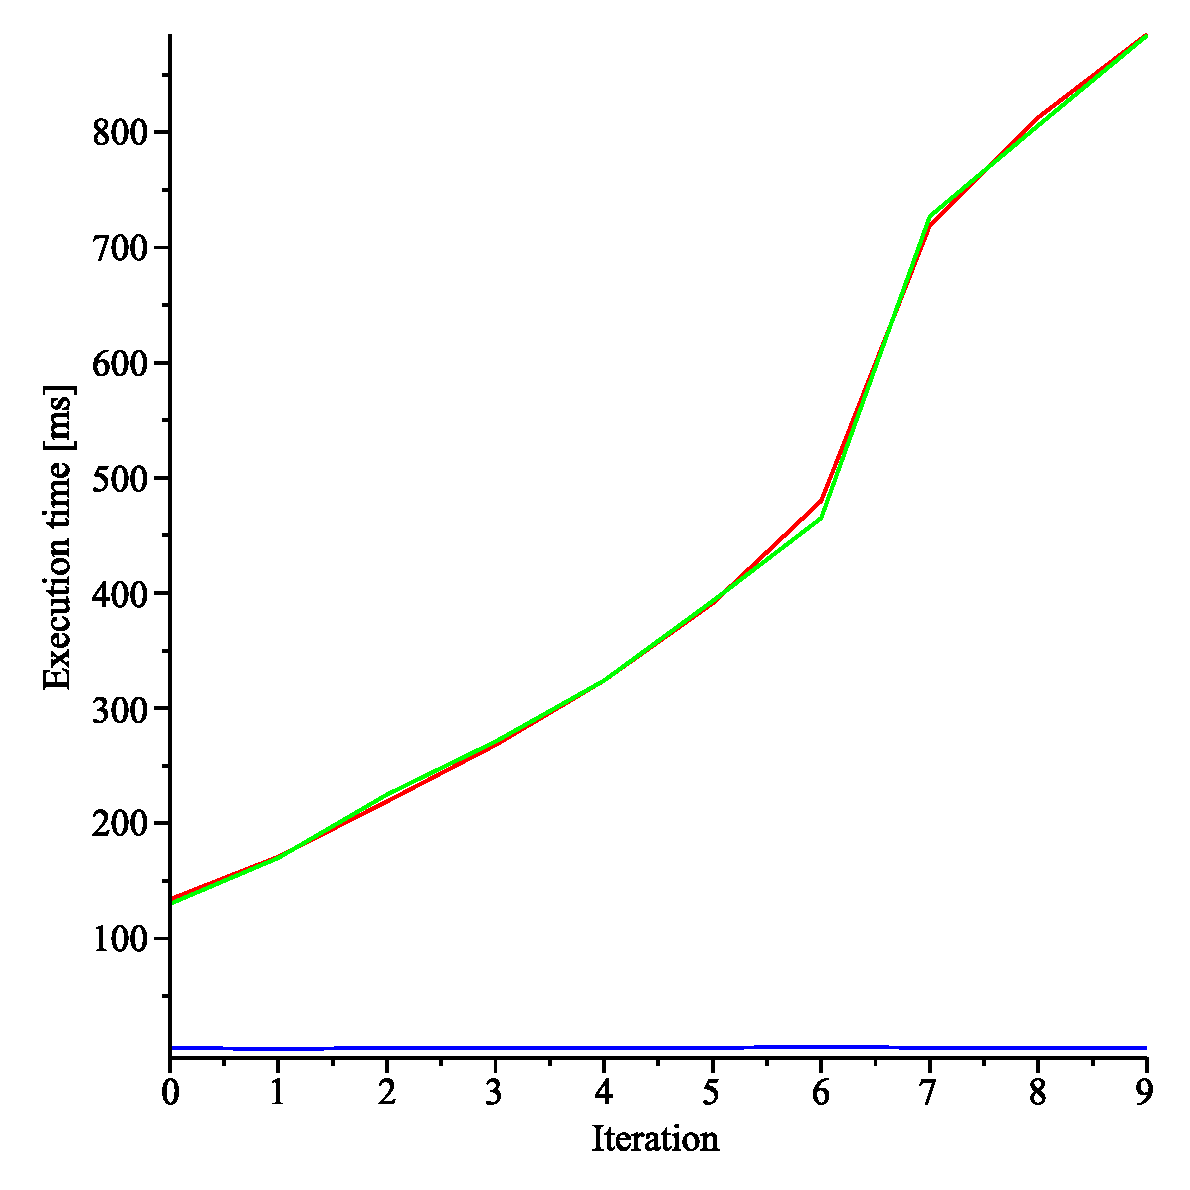
\includegraphics[width=1\textwidth]{alfp_graph.eps}

The red line executions times for the differential algorithm, the blue line is our implementation, and the green line is the BDD based algorithm. The values can be seen in appendix 7.6.

As the graph shows, the time for our implementation is very close to constant in this test, while the time for both algorithms rises. Something strange happens between execution 7 and 8, as the time jumps with just over 200 ms. It was also about that point where it took up to 10 executions before the time were as low as those in the graph. Instead, the execution time would be somewhere from 1000 ms to 4000 ms, and usually about 1400 ms. Perhaps the size of storing the calculations which needed to be done on the clauses, became higher than what the kernel wanted to cache, and therefore it had to load in the rest of the calculations before it could continue. Perhaps it had to rehash everything because the number of clauses where higher than there were space for. No matter what the reason is, the use of the succinct solver is still the slowest solution to use.



\chapter{Evaluation}


In the project, a program analysis module has been implemented.
Below, the different parts will be discussed.

\paragraph{Analyses:}
The 3 required analyses have been implemented in the project,
and the theory behind them have been described. Of note is that
SLVA has been implemented, to provide a more precise analysis
and a more effective Dead Code Elimination. We believe that SLVA
is important for the performance of DCE, since it frequently gives
a much more precise transformation. An example is given where LVA
keeps resurrecting faint variables, which should be removed, while
SLVA marks them as dead.

The constant propagation
has furthermore been given support for branch killing, which is also
quite useful. Killing branches can occur quite often in programs, for
instance in the case that a branch containing debug-code/test code
is killed because its condition is set to false (for instance through
a global constant).

The analyses have been tested by hand, but not through automated tests.
Besides this testing, they have been tested indirectly through the
transformations, because the transformations rely on the analyses being
correct.

Given the testing of the analyses and the performance of the transformations,
it is estimated that the analyses have been defined and implemented correctly.
Given the time frame and scope of the project, this is deemed sufficient
regarding the correctness of the analyses.

\paragraph{Transformations:}
The 3 required transformations, Program Slicing, Dead Code Elimination
and Constant Propagation, have been fully implemented.

Program Slicing is deemed to being implemented correctly, based on the
tests performed. The definition of PS can vary a lot, but it is deemed
that the definition in this project is both useful and somewhat simple.
This is confirmed by the implementation of PS. The definitionen not only
shows the relevant parts, but also preserves a runnable program, which
may be useful. Some other groups' definition of PS varies from this definition,
some ignoring control flow and focusing solely on the RD.
We believe that this definition gives a more usable PS, but this may depend
on the purpose of the PS. The purposes can include debugging for the
programmer, which suits this definition well.

The Dead Code Elimination is deemed to be very useful internally in regards
to cleaning up from other transformations. While it is rare for programmers
not to use variables, transformations frequently do not clean up after themselves,
including PS and CF. Another use for DCE is marking code for the programmer
that is dead, which although rare may indicate bugs.

The Constant Folding is deemed to be quite useful, especially given its
branch killing. As mentioned in the evaluation of the analyses,
branch killing can remove considerable parts of the code that ends up
in the final result, but can also increase the speed of the analyses and
transformations in general, because dead code is not investigated with
branch killing.

It is deemed that all the transformations perform well, and that they
have been tested well with both general programs and special case programs.

\paragraph{Worklist:}
The worklist implemented has focused less on generalisation, and more
on efficiency. In this regard, the worklist has performed admirably.
As seen in the test regarding the Succint Solver, it outperforms
the other methods, especially when the problem instances scales.

This comes at a price in generality. However, it is deemed that
this price is acceptable for multiple reasons: it shows that a worklist
implemented for specific problem instances can severely outperform
general implementations; and it gives a much better performance.

\paragraph{Testing:}

The testing is based on regression-testing. This means that the precise expected
output is written by the tester, and the test then succeeds only if the resulting
output is exactly the same as the expected output. This may result in false positives:
results that are correct but not the same as the expected will be registered as positives.
While this is not optimal, it is considered acceptable. Partly since implementing tests other
than regression tests is outside the scope of the project, and partly since the current
transformations implemented produce the same output if they are correct.



\chapter{Conclusion}


In this project, a program analysis module have been
designed, implemented and tested. A theoretical background
have been given for the analyses, and the Succinct Solver
has been tested against the worklist in the project.

\paragraph{Analyses:}

All the required assignments regarding analyses have been performed.

The analyses have been given a theoretical background,
and is deemed to be defined and implemented correctly,
given the testing and the performance of the transformations.
Of note is the implementation of Strongly Live Variable Analysis,
giving a considerably better performance than the simpler Live Variable Analysis,
and the Constant Propagation branch killing, enabling removal of dead code based on branches.

Both SLVA and CP branch killing is recommended, since the authors
believe that their increased performance outweights the required
definition and work.

\paragraph{Transformations:}

All the required assignments regarding transformations have been performed.
The transformations have been defined, designed, implemented and tested.

The Program Slicing has been examined thoroughly, and given a definition which should
make the PS useful for debugging as well as other purposes. It has
been compared with other groups, and is considered to have performed
well, as well as following the definition given. The given definition of PS has not
been used in real life, and can therefore not be recommended at the given point in time.
We recommend investigating the use of PS more, possibly test PS, to decide which
definition of PS is useful and in which cases.

The Dead Code Elimination performs well, and benefits well from the SLVA. It has
been deemed to be useful to clean up dead code from other transformations,
and could be used to indicate dead code for the programmer. LVA is not guaranteed to
perform as well as SLVA, even through repeated runs. For projects
implementing DCE, SLVA is therefore strongly recommended.

The Constant Folding performs well, especially given the branch killing. As argued,
dead branches occur in both programmers code and internally after transformations,
which makes branch killing especially useful. Not only does this have the potential
to make the analyses more precise, it can also decrease the program size that have
to be considered. Based on this, we recommended Constant Folding.

\paragraph{Worklist:}
As seen in the comparsion with the Succinct Solver, the worklist performs admirably.
For the same problem instances, the efficiency difference is quite large, and the
results are the same. Based on this, it is our recommendation that whenever a
general solution vs. a performance-tuned solution regarding worklists is considered,
the performance of the general solution must be carefully evaluated. If it does not
fulfill the needs for efficiency, it may be fruitful to find/implement a more
specific solution.

The main disadvantage is the lack of generality. This means that this implementation
may have less uses without adaptation. However, the worklist is both useful and can
be used as a benchmark between general solutions and more specific solutions,
which may be useful given that GCL is a somewhat simple language.

\paragraph{General conclusion:}
It is estimated that the project is successful. All assignments have
been completed, and more parts than required in the assignment have been added,
including branch killing.



\chapter{Appendix}

\section{Abbreviations and acronyms}

This section contains a list of abbreviations and acronyms used in
the report.

\begin{itemize}
\item CP(A) - Constant Propagation (Analysis)
\item GCC - GNU Compiler Collection (or GNU C Compiler)
\item GCL - Guarded Command Language
\item IR - Intermediate (or Internal) Representation
\item LV(A) - Live Variable (Analysis)
\item RD(A) - Reaching Definitions (Analysis)
\item SLV(A) - Strongly Live Variable (Analysis)
\end{itemize}

\section{Test results}



\end{document}

